\section{Design Space}
\label{sec:dspace}

The narrow interface exposed by storage systems has been a boon in allowing
systems and applications to evolve independently, in affect limiting the size
of the design space where applications couple with storage. Programmable
storage lifts the veil on the system, and with it, forces applications developers
to confront a large set of possible designs.

\subsection{Software Parameters}

To illustrate the design space challenge we implemented as an object interface
the CORFU storage device specification, that is a write-once interface over a
64-bit address space. The interface is used as a building block of the CORFU
protocol to read and write log entries that are striped over an entire
cluster.  The implementations differ in their optimization strategy of
utilizing internal system interfaces. For instance one implementation uses a
key-value interface to manage the address space index and entry data, while
another implementation stores the entry data using a byte-addressable
interface.

\begin{figure}[t]
\centering
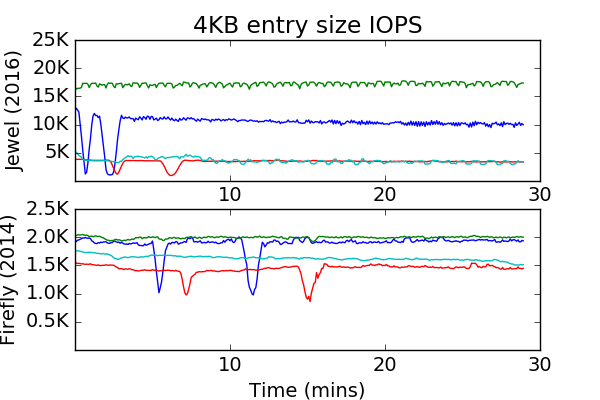
\includegraphics[width=1.0\linewidth]{jewel_v_firefly_pd.png}
\caption{asdf}
\label{fig:phy-design}
\end{figure}

Figure~\ref{fig:phy-design} shows the append throughput of four such
implementations run on two versions of Ceph from 2014 and 2016. The first
observation to be made is that performance in general is significantly better
in the newer version of Ceph. However, what is interesting is the relationship
between the implementations. Run on a version of Ceph from 2014, the top two
implementations perform with nearly identical throughput, but have strikingly
different implementation complexities. The performance of the same
implementations on a newer version of Ceph illustrate a challenge: given a
reasonable choice of a simpler implementation in 2014, a storage interface
will perform worse in 2016, requiring significant rework of low-level
interface implementations.

\textbf{Takeaway}: Choosing the best implementations is dependent on both the
timing of the development (Ceph Version) and the expertise of the
administrator (Ceph Features). Ceph development is a moving target with
multiple stable releases each year, 400+ contributors, and 70--260 commits per
week.  Disruptive and innovative change in Ceph is also common place, with
features such as BlueStore~\cite{weil:vault2016-bluestore} replacing
traditional file systems like XFS that have limitations on the workloads
generated by Ceph such as double writes and metadata scalability. 

\subsubsection{System Tunables}

The most recent version of Ceph (v10.2.0-1281-g1f03205) has 994 tunable
parameters\footnote{This number comes from \texttt{src/common/config\_opts.h}
with debug options filtered out.}, where 195 of them pertain to the OSD itself
and 95 of them focus on the OSD back end file system (i.e. its
\texttt{filestore}). Ceph also has tunables for the subsystems it uses, like
LevelDB (10 tunables), RocksDB (5 tunables), its own key-value stores (5
tunables), its object cache (6 tunables), its journals (24 tunables), and its
other optional object stores like BlueStore (49 tunables).

This many domain-specific tunables makes it almost impossible to come up with
the best set of tunables, although auto-tuning like the work done
in~\cite{behzad:sc2013-autotuning} could go a long way. Regardless of the
technique that we use, it is clear the number of tunables increases the
physical design parameters to an unwieldy state space size.

\textbf{Takeaway}: the number and complexity of Ceph's tunables makes
brute-force parameter selection hard.

\subsubsection{Hardware Parameters}

Ceph is designed to run on a wide variety of commodity hardware as well as new
NVMe devices. All these devices have their own set of characteristics and
tunables (e.g., the IO operation scheduler type). In our experiments, we tested
SSD, HDDs, NVMe devices and discovered a wide range of behaviors and
performance profiles. As an example, Figure~\ref{fig:jewel-hdd-128b} shows the
write performance of 128 byte log entries using Jewel and a single HDD.
Performance is 10\(\times\) slower than its SSD counterpart in
Figure~\ref{fig:jewel_v_firefly_v_es} (top row, third column) but the behavior
and relative performance make this hardware configuration especially tricky.

The behavior of the 1:1 implementations shows throughput drops lasting for
minutes at a time -- this limits our focus to the N:1 implementations. The
performance of \texttt{(N:1, BS)} implementation is almost identical to
\texttt{(N:1, KV)} (within 1\% mean throughput). Regardless of the true
bottleneck, it is clear that choosing \texttt{(N:1, KV)} is the better choice
because of the resulting implementation should be less complex and there is
minimal performance degradation.

\textbf{Takeaway}: choosing the best implementations is dependent on hardware.
Something as common as an upgrade from HDD to SSD may nullify the benefits of a
certain implementation. 
